\documentclass[a4paper,12pt]{scrreprt}

\usepackage[utf8x]{inputenc}
\usepackage{ucs}
\usepackage{graphicx}
\usepackage[ngerman,english]{babel} %% NOTE: The *last* language is the active one!
                                    %% See babel documentation for further details.
\usepackage{acronym}
\usepackage{eurosym}
\usepackage[linktocpage=true]{hyperref}
\usepackage{caption}
\captionsetup{format=hang, justification=raggedright}
\usepackage[sort]{natbib} % vgl. http://merkel.zoneo.net/Latex/natbib.php

\setcounter{secnumdepth}{4}
\setcounter{tocdepth}{4}


\begin{document}

\pagenumbering{gobble} % suppress page numbers

% perhaps a restriction note
If required (only in reasonable cases): restriction note

% title page:
\newpage
\pagenumbering{arabic} % begin with page numbering
\begin{titlepage}
  \mbox{}
  \vspace{5mm}
  \begin{center}
    \huge{\textbf{\sffamily[TITLE OF THE THESIS]}} \\
    \huge{\textbf{\sffamily[if required: sub title]}}\\
  \end{center}
  \vspace{40mm}
  \begin{flushright}
  Bachelor thesis [1 or 2]\\
  to obtain the academic degree\\
  \textbf{Bachelor of Science in Engineering (BSc)}

  \vspace{20mm}
  Fachhochschule Vorarlberg\\
  Informatics

  \vspace{40mm}
  Filed with\\\relax
  Prof. Dr. Bla di Blub\\
  Submitted by\\\relax
  academic degree of student\\

  \vspace{20mm}
  Dornbirn, [Month Year]
  \end{flushright}
\end{titlepage}

\chapter*{[If required: Dedication]}

% Abstract:
\newpage
\chapter*{Abstract}
Style sheet for a continuous text

% evtl. Vorwort:
\newpage
\chapter*{[If required: Preface]}


% directories

\tableofcontents

\clearpage
\phantomsection
\addcontentsline{toc}{chapter}{List of Figures}
\listoffigures

\clearpage
\phantomsection
\addcontentsline{toc}{chapter}{List of Tables}
\listoftables

% perhaps a list of abbreviations:
\newpage
\chapter*{[If required: List of Abbreviations]}
\begin{acronym}[SQL]
 \acro{KDE}{K Desktop Environment}
 \acro{SQL}{Structured Query Language}
 \acro{Bash}{Bourne-again shell}
\end{acronym}

% end of: directories

% define and add/include you chapters and/or sections here.
% be aware though, paths are relative to 'main.tex'
\chapter{Introduction}
Lorem ipsum dolor sit amet, consetetur sadipscing elitr, sed diam nonumy
eirmod tempor invidunt ut labore et dolore magna aliquyam erat, sed diam
voluptua. At vero eos et accusam et justo duo dolores et ea rebum. Stet
clita kasd gubergren, no sea takimata sanctus est Lorem ipsum dolor sit
amet. Lorem ipsum dolor sit amet, consetetur sadipscing elitr, sed diam
nonumy eirmod tempor invidunt ut labore et dolore magna aliquyam erat, sed
diam voluptua. At vero eos et accusam et justo duo dolores et ea rebum.
Stet clita kasd gubergren, no sea takimata sanctus est Lorem ipsum dolor
sit amet.

\begin{quote}

    Lorem ipsum dolor sit amet, consetetur sadipscing elitr, sed diam
    nonumy eirmod tempor invidunt ut labore et dolore magna aliquyam erat,
    sed diam voluptua. At vero eos et accusam et justo duo dolores et ea
    rebum. Stet clita kasd gubergren, no sea takimata sanctus est Lorem
    ipsum dolor sit amet. Lorem ipsum dolor sit amet, consetetur sadipscing
    elitr, sed diam nonumy eirmod...

\end{quote}

Guides on how to quote using external sources can be found via  \glqq
Wissenschaftliches Arbeiten. Ein Leitfaden\grqq. The latest version can be
found on FHV-Bibliothekshomepage and downloaded for free
(\href{http://www.fhv.at/bibliothek/teaching-library/leitfaden}{http://www.fhv.at/bibliothek/teaching-library/leitfaden}).

\chapter{Main Part}
Lorem ipsum dolor sit amet, consetetur sadipscing elitr, sed diam nonumy
eirmod...

A list
\begin{enumerate}
 \item understand
 \item practise
 \item being capable of
\end{enumerate}


\section{Subchapter: second level}

Style sheet for continuous text. The figure~\ref{fig:ex} on page \pageref{fig:ex}
illustrates three drain curves of a two-phase defibrillator.

\begin{figure}[htb]
  \centering
  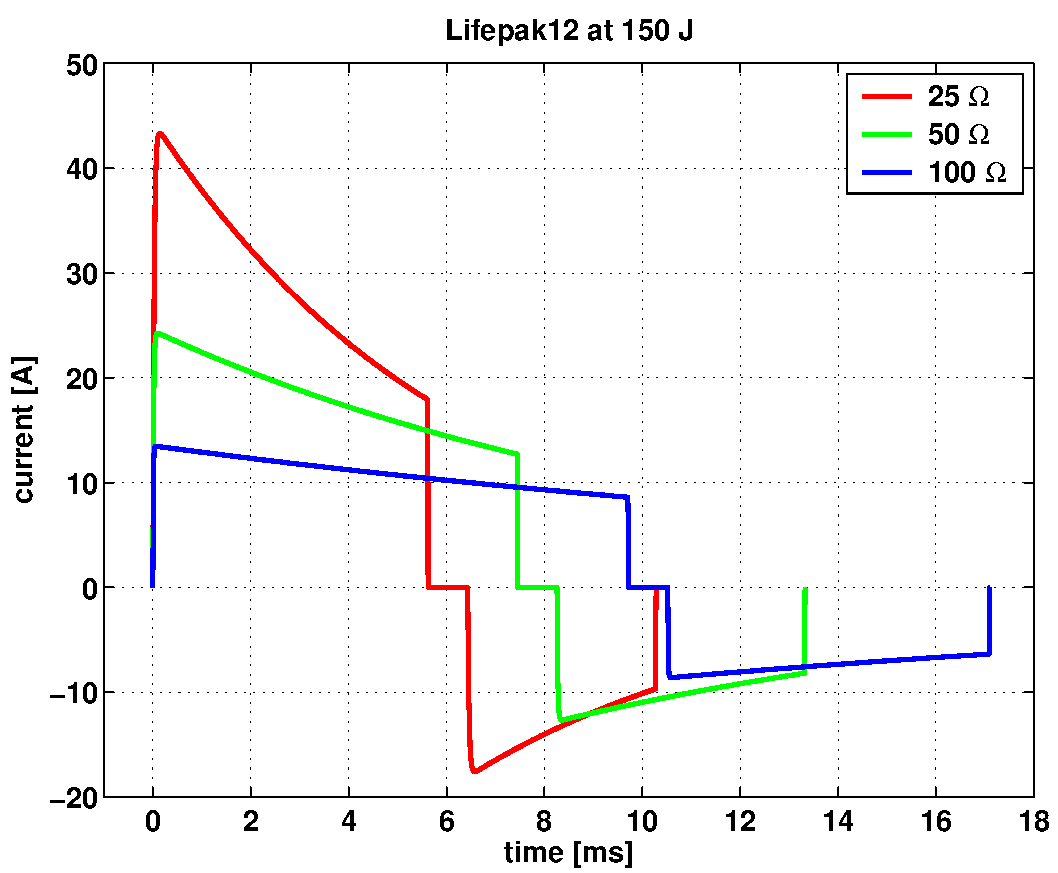
\includegraphics[width=6cm]{content/image/defi}
  \caption[Drain curve of a two-phase defibrillator]{Three drain curves. \\Source: own elaboration}
 \label{fig:ex}
\end{figure}


\section{Subchapter: second level}
Style sheet for continuous text. .
Now a footnote\footnote{This is a footnote.}
How many roots does the quadratic equation (\ref{equ:foo}) has?
\begin{equation}
 \label{equ:foo}
 x^2-2x+5=0.
\end{equation}
Two of Einsteins' most famous equations:
\begin{eqnarray*}
  E &= mc^2                                  \\
  m &= \frac{m_0}{\sqrt{1-\frac{v^2}{c^2}}}
\end{eqnarray*}


\subsection{Subsection third level}
Style sheet for continuous text. A simple table \ref{tab:sp} follows

\begin{table}[htb]
  \centering
  \begin{tabular}{ | l | l |c|}
    \hline
    Date      & Topic           & Room \\
    \hline\hline
    Monday     & Graph theory  & U1   \\
    \hline
    Thursday & Algebra         & MZB23\\
    \hline
  \end{tabular}
  \caption[Timetable]{Timetable of 2030.\\ Source: own elaboration}
  \label{tab:sp}
\end{table}

\subsubsection{Subsection: fourth level}
Style sheet for continuous text.

\paragraph{Subsection: fifth level}\mbox{}\newline
Style sheet for continuous text.

\paragraph{Subsection: fifth level}\mbox{}\newline
Style sheet for continuous text.


\section{Subchapter: second level}
Style sheet for continuous text. .
A recommended book \citep[vgl.][Chapter 2]{Chvatal1983} and an interesting article \citep{Einstein1905} of a famous man.


\chapter{[Another Chapter of the Main Part]}

\section{Subchapter: second level}
Style sheet for continuous text.

\subsection{Subchapter: third level}
Style sheet for continuous text.

\subsubsection{Subchapter: fourth level}
Style sheet for continuous text.

\paragraph{Subchapter: fifth level}\mbox{}\newline
Style sheet for continuous text.

\paragraph{Subchapter: fifth level}\mbox{}\newline
Style sheet for continuous text.


\chapter{[Last chapter]}
Style sheet for continuous text.



% \bibliographystyle{unsrt}
% \bibliographystyle{alpha}
% \bibliographystyle{plain}
% \bibliographystyle{unsrtnat}
\bibliographystyle{authordate3}
\clearpage
\phantomsection
\addcontentsline{toc}{chapter}{Bibliography}
\bibliography{references} % references.bib is the used bibtex file


\chapter*{[If required: Attachment]}
\addcontentsline{toc}{chapter}{[If required: Attachment]}
Style sheet for a continuous text

\chapter*{Statutory Declaration}
\addcontentsline{toc}{chapter}{Statutory Declaration}

I hereby declare that I have authored this thesis independently, that I
have not used other than the declared sources/resources, and that I have
explicitly marked all material which has been quoted either literally or by
content from the used sources.

\vfill

%% definition of the block tat contains date and signature
\newcommand{\mysignatureblock}[3]{%
  %% Sorry, this is a "bit" of a hack. Maybe someone knows a more elegant method?
  \begin{tabular}{llp{2em}l}
  #1 & \hspace{4cm}        & & \hspace{5cm} \\\cline{2-2}\cline{4-4}
     &                     & & \\[-3mm]
     & {\footnotesize #2}  & & {\footnotesize #3}
  \end{tabular}
}

\mysignatureblock{Dornbirn,}{Date}{Fore- and Surname}

\vfill\vfill


\end{document}
